\chapter{Máquinas de vectores de soporte}\label{Chapter8} 
% chktex-file 8
% chktex-file 12
% chktex-file 13
% chktex-file 44

Se ha demostrado que las SVMs funcionan bien en una variedad de entornos y a menudo se consideran uno de los mejores clasificadores ``listos para usar''. \\

La máquina de vectores de soporte es una generalización de un clasificador simple e intuitivo llamado clasificador de máximo margen, Aunque es elegante y simple,  este clasificador no se puede aplicar a la mayoría de los conjuntos de datos, ya que requiere que las clases sean separables por un límite lineal. El clasificador de vectores de soporte es una extensión del clasificador de máximo margen que se puede aplicar en una gama más amplia de casos. Finalmente, la máquina de vectores de soporte es una extensión adicional del clasificador de vectores de soporte para acomodar límites de clase no lineales. Las máquinas de vectores de soporte están destinadas al entorno de clasificación binaria en el que hay dos clases. 

\section{Clasificador de máximo margen}

\subsection{Hiperplano}

En un espacio p-dimensional, un hiperplano es un subespacio afín plano de dimensión $p - 1$. Por ejemplo, en dos dimensiones, un hiperplano es un subespacio plano unidimensional, en otras palabras, una línea. En tres dimensiones, un hiperplano es un subespacio plano bidimensional, es decir, un plano. La definición matemática de un hiperplano es bastante simple. En dos dimensiones, un hiperplano se define por la ecuación
\begin{equation}
\beta_0 + \beta_1 X_1 + \beta_2 X_2 = 0
\label{eq:9.1}
\end{equation}

para los parámetros $\beta_0$, $\beta_1$ y $\beta_2$. Cuando decimos que esta ecuación define el hiperplano, queremos decir que cualquier $X = (X_1, X_2)^T$ para el cual se cumple esta ecuación es un punto en el hiperplano. La ecuación anterior puede extenderse fácilmente al entorno p-dimensional:
\begin{equation}
\beta_0 + \beta_1 X_1 + \beta_2 X_2 + \ldots + \beta_p X_p = 0
\label{eq:9.2}
\end{equation}

define un hiperplano p-dimensional, nuevamente en el sentido de que si un punto $X = (X_1, X_2, \ldots, X_p)^T$ en el espacio p-dimensional (es decir, un vector de longitud $p$) satisface esta ecuación, entonces $X$ se encuentra en el hiperplano. \\

\noindent Ahora, supongamos que $X$ no satisface la ecuación (\ref{eq:9.2}); más bien,
\begin{equation}
\beta_0 + \beta_1 X_1 + \beta_2 X_2 + \ldots + \beta_p X_p > 0.
\end{equation}

\noindent Entonces esto nos dice que $X$ se encuentra a un lado del hiperplano. Por otro lado, si
\begin{equation}
\beta_0 + \beta_1 X_1 + \beta_2 X_2 + \ldots + \beta_p X_p < 0,
\end{equation}

entonces $X$ se encuentra al otro lado del hiperplano. Así que podemos pensar en el hiperplano como una divisón del hiperespacio en dos mitades. Uno puede determinar fácilmente en qué lado del hiperplano Un hiperplano en el espacio bidimensional se muestra en la figura \ref{fig:9.1}.

\begin{figure}[h]
\centering
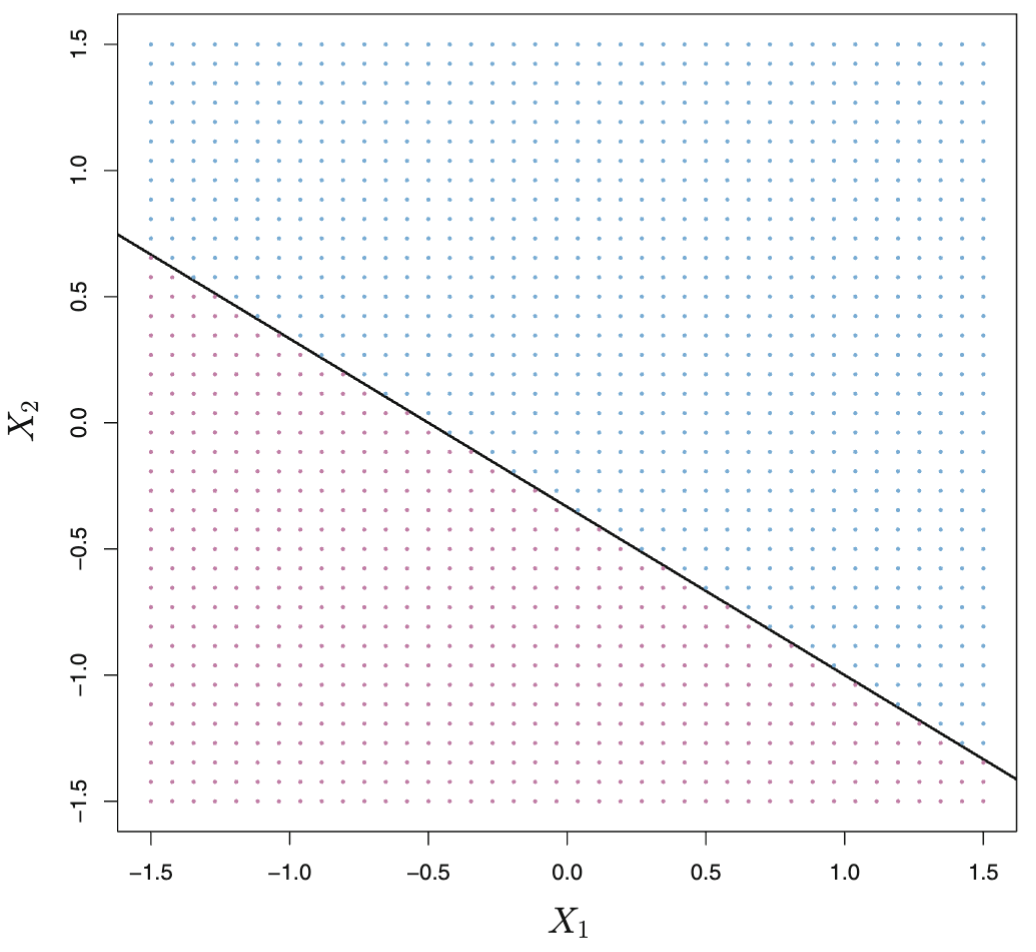
\includegraphics[width=0.5\textwidth]{fotos/52.png}
\caption{Hiperplano $1 + 2X_1 + 3X_2 = 0$. La región azul consiste en los puntos tales que $1 + 2X_1 + 3X_2 > 0$, mientras que la región roja consiste en los puntos tales que $1 + 2X_1 + 3X_2 < 0$.}
\label{fig:9.1}
\end{figure}

\subsection{Clasificación usando un hiperplano separador}

Ahora supongamos que tenemos una matriz de datos $n \times p$ $\mathbf{X}$ consistente en $n$ observaciones de entrenamiento en un espacio p-dimensional,
\begin{equation}
x_1 =
\begin{pmatrix}
x_{11} \\
\vdots \\
x_{1p}
\end{pmatrix}, \ldots, x_n =
\begin{pmatrix}
x_{n1} \\
\vdots \\
x_{np}
\end{pmatrix},
\end{equation}
y que estas observaciones caen en dos clases, es decir, $y_1, \ldots, y_n \in \{-1, 1\}$ donde $-1$ representa una clase y $1$ la otra clase. También tenemos una observación de prueba, un vector p-dimensional de características observadas $x^* = (x^*_1, \ldots, x^*_p)^T$. Nuestro objetivo es desarrollar un clasificador basado en los datos de entrenamiento que clasifique correctamente la observación de prueba utilizando sus mediciones de características. Lo haremos con un nuevo enfoque basado en el concepto de un hiperplano separador. \\

\begin{figure}[h]
\centering
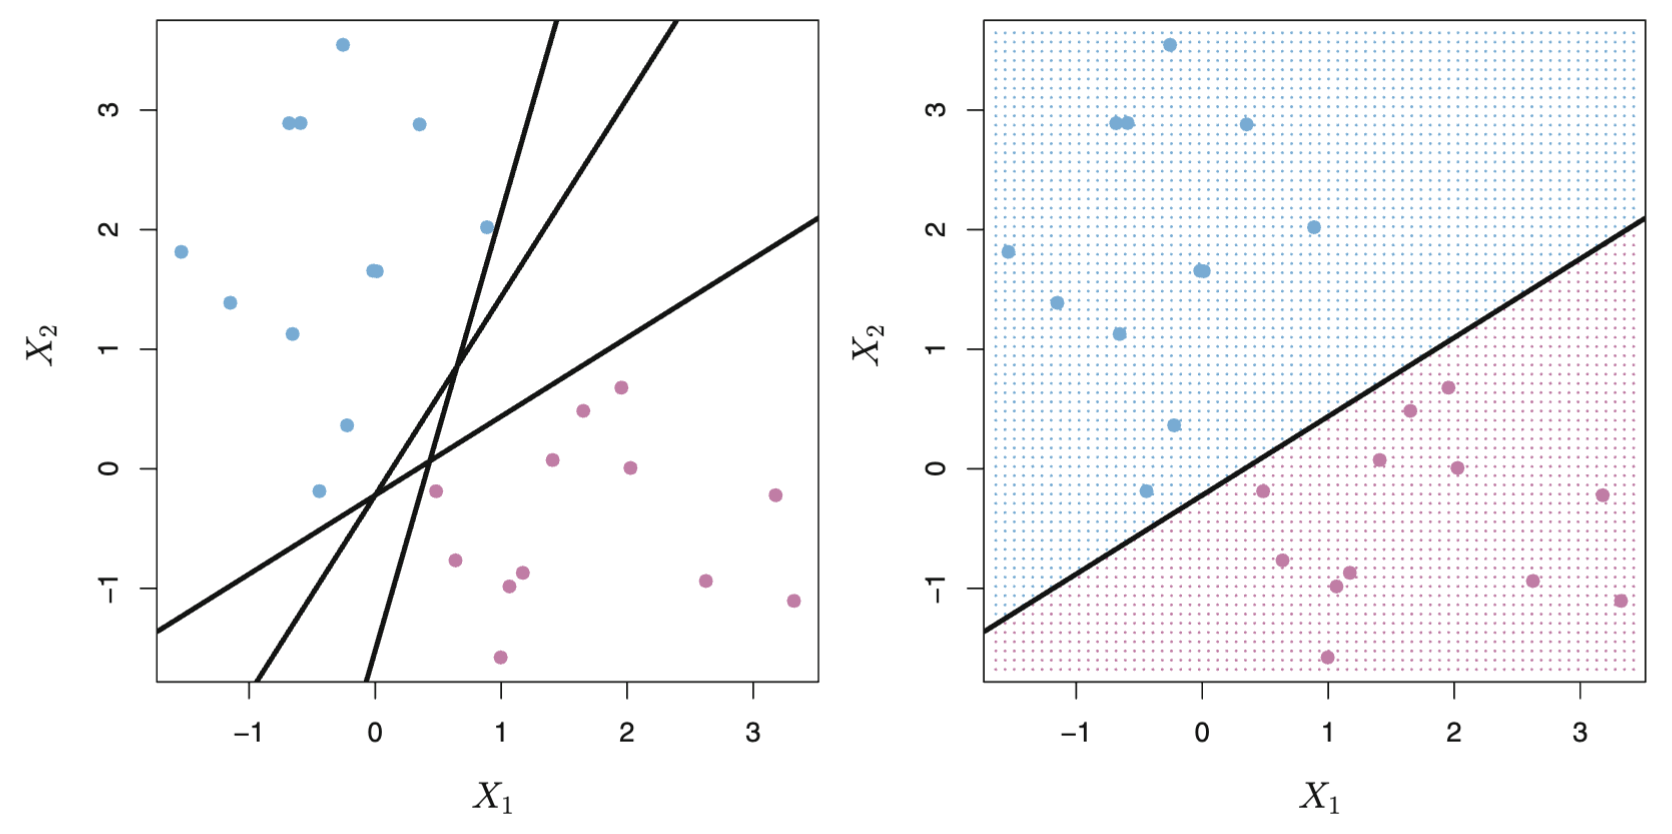
\includegraphics[width=\textwidth]{fotos/53.png}
\caption{Izquierda: hay dos clases de observaciones (en distintos colores), cada una con medidas en dos variables. Se muestran tres posibles hiperplanos separadores en negro. Derecha: se muestra un ejemplo de hiperplano separador, los ejemplos que caigan en la zona azul serán clasificados como esa clase, mientras que los que caigan en la región morada, serán clasificados como de esa clase.}
\label{fig:9.2}
\end{figure}

Supongamos que es posible construir un hiperplano que separe perfectamente las observaciones de entrenamiento según sus etiquetas de clase. Ejemplos de tres de estos hiperplanos separadores se muestran en el panel izquierdo de la figura \ref{fig:9.2}. Podemos etiquetar las observaciones de la clase azul como $y_i = 1$ y las de la clase púrpura como $y_i = -1$. Entonces, un hiperplano separador tiene la propiedad de que
\begin{align}
\beta_0 + \beta_1 x_{i1} + \beta_2 x_{i2} + \ldots + \beta_p x_{ip} > 0 &\text{ si } y_i = 1, \\
\beta_0 + \beta_1 x_{i1} + \beta_2 x_{i2} + \ldots + \beta_p x_{ip} < 0 &\text{ si } y_i = -1.
\end{align}

\noindent De manera equivalente, un hiperplano separador tiene la propiedad de que
\begin{equation}
y_i (\beta_0 + \beta_1 x_{i1} + \beta_2 x_{i2} + \ldots + \beta_p x_{ip}) > 0
\end{equation}

\noindent para todo $i = 1, \ldots, n$. \\

Si existe un hiperplano separador, podemos usarlo para construir un clasificador muy natural: una observación de prueba se asigna a una clase dependiendo de en qué lado del hiperplano se encuentra. El panel derecho de la figura \ref{fig:9.2} muestra un ejemplo de tal clasificador. Es decir, clasificamos la observación de prueba $x^*$ basándonos en el signo de 
\begin{equation}
f(x^*) = \beta_0 + \beta_1 x^*_1 + \beta_2 x^*_2 + \ldots + \beta_p x^*_p
\end{equation}

Si $f(x^*)$ es positivo, entonces asignamos la observación de prueba a la clase 1, y si $f(x^*)$ es negativo, entonces la asignamos a la clase -1. También podemos hacer uso de la magnitud de $f(x^*)$. Si $f(x^*)$ está lejos de cero, esto significa que $x^*$ está lejos del hiperplano, por lo que podemos estar seguros de nuestra asignación de clase para $x^*$. Por otro lado, si $f(x^*)$ está cerca de cero, entonces $x^*$ está cerca del hiperplano, por lo que estamos menos seguros de la asignación de clase para $x^*$. Un clasificador basado en un hiperplano separador conduce, por tanto, a un límite de decisión lineal.

\subsection{Clasificador de máximo margen}

En general, si nuestros datos pueden ser perfectamente separados usando un hiperplano, entonces existirá un número infinito de tales hiperplanos. Para construir un clasificador basado en un hiperplano separador, debemos tener una forma razonable de decidir cuál de los infinitos hiperplanos separadores posibles usar. \\

Una elección natural es el hiperplano de máximo margen (también conocido como el hiperplano separador óptimo), que es el hiperplano separador que está más alejado de las observaciones de entrenamiento. Es decir, podemos calcular la distancia (perpendicular) desde cada observación de entrenamiento hasta un hiperplano separador dado; la menor de estas distancias es la distancia mínima desde las observaciones hasta el hiperplano, y se conoce como el margen. El hiperplano de máximo margen es el hiperplano separador para el cual el margen es mayor, es decir, es el hiperplano que tiene la mayor distancia mínima a las observaciones de entrenamiento. Luego podemos clasificar una observación de prueba según el lado del hiperplano de máximo margen en el que se encuentre. Esto se conoce como el clasificador de máximo margen. Esperamos que un clasificador que tenga un gran margen en los datos de entrenamiento también tenga un gran margen en los datos de prueba, y por lo tanto clasifique correctamente las observaciones de prueba. Aunque el clasificador de máximo margen a menudo tiene éxito, también puede llevar a un sobreajuste cuando $p$ es grande. \\

Si $\beta_0, \beta_1, \ldots, \beta_p$ son los coeficientes del hiperplano de máximo margen, entonces el clasificador de margen máximo clasifica la observación de prueba $x^*$ basándose en el signo de $f(x^*) = \beta_0 + \beta_1 x^*_1 + \beta_2 x^*_2 + \ldots + \beta_p x^*_p$. \\

\begin{figure}[h]
\centering
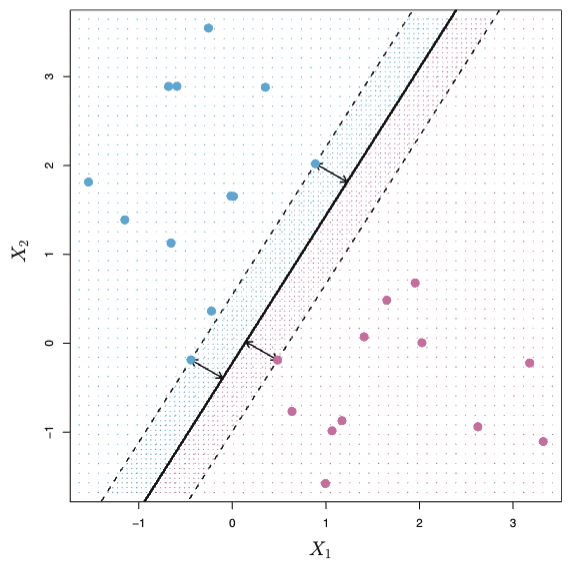
\includegraphics[width=0.5\textwidth]{fotos/54.png}
\caption{Hiperplano de margen máximo.}
\label{fig:9.3}
\end{figure}

La figura \ref{fig:9.3} muestra el hiperplano de margen máximo en el conjunto de datos de la figura \ref{fig:9.2}. Comparando el panel derecho de la figura \ref{fig:9.2} con la figura \ref{fig:9.3}, vemos que el hiperplano de margen máximo mostrado resulta en una mayor distancia mínima entre las observaciones y el hiperplano separador, es decir, un margen mayor. \\

Examinando la figura \ref{fig:9.3}, vemos que tres observaciones de entrenamiento son equidistantes al hiperplano de máximo margen y se encuentran a lo largo de las líneas discontinuas que indican el ancho del margen. Estas tres observaciones se conocen como vectores de soporte, ya que son vectores en el espacio p-dimensional (en esta figura, $p = 2$) y "soportan" el hiperplano de máximo margen en el sentido de que si estos puntos se movieran ligeramente, el hiperplano también se movería. Así, el hiperplano de margen máximo depende directamente de los vectores de soporte, pero no de las otras observaciones: un movimiento de cualquiera de las otras observaciones no afectaría el hiperplano separador, siempre que el movimiento de la observación no cause que cruce el límite establecido por el margen. \\

\subsection{Construcción del clasificador de máximo margen}

Ahora consideramos la tarea de construir el hiperplano de máximo margen basado en un conjunto de $n$ pares de observaciones de entrenamiento $(x_1, y_1) (x_2, y_2), \ldots, (x_n, y_n)$, donde $x_i \in \mathbb{R}^p$ y las etiquetas de clase asociadas $y_i \in \{-1, 1\}$. Brevemente, el hiperplano de margen máximo es la solución al problema de optimización
\begin{align}
\underset{\beta_0, \beta_1, \ldots, \beta_p}{\text{Maximizar }} & M \label{eq:9.9}\\
\text{sujeto a } & \sum_{j = 1}^{p} \beta_j^2 = 1, \label{eq:9.10}\\
& y_i (\beta_0 + \beta_1 x_{i1} + \beta_2 x_{i2} + \ldots + \beta_p x_{ip}) \geq M \quad \forall i = 1, \ldots, n \label{eq:9.11}
\end{align}

\noindent Este problema de optimización es simple. En primer lugar, la restricción 
\begin{equation}
y_i (\beta_0 + \beta_1 x_{i1} + \beta_2 x_{i2} + \ldots + \beta_p x_{ip}) \geq M \quad \forall i = 1, \ldots, n
\end{equation}

garantiza que cada observación estará en el lado correcto del hiperplano, siempre que $M$ sea positivo. De hecho, para que cada observación esté en el lado correcto del hiperplano, simplemente necesitaríamos $y_i (\beta_0 + \beta_1 x_{i1} + \beta_2 x_{i2} + \ldots + \beta_p x_{ip}) > 0$, por lo que la restricción requiere que cada observación esté en el lado correcto del hiperplano, con un cierto margen, siempre que $M$ sea positivo. \\

En segundo lugar, observe que (\ref{eq:9.10}) no es realmente una restricción sobre el hiperplano, ya que si $\beta_0 + \beta_1 x_{i1} + \beta_2 x_{i2} + \ldots + \beta_p x_{ip} = 0$ define un hiperplano, entonces también lo hace $k (\beta_0 + \beta_1 x_{i1} + \beta_2 x_{i2} + \ldots + \beta_p x_{ip}) = 0$ para cualquier $k \neq 0$. Sin embargo, (\ref{eq:9.10}) añade significado a (\ref{eq:9.11}); se puede demostrar que, con esta restricción, la distancia perpendicular desde la $i$-ésima observación al hiperplano está dada por
\begin{equation}
y_i (\beta_0 + \beta_1 x_{i1} + \beta_2 x_{i2} + \ldots + \beta_p x_{ip}).
\end{equation}
Por lo tanto, las restricciones (\ref{eq:9.10}) y (\ref{eq:9.11}) aseguran que cada observación esté en el lado correcto del hiperplano y al menos a una distancia $M$ del hiperplano. Por lo tanto, $M$ representa el margen de nuestro hiperplano, y el problema de optimización elige $\beta_0, \beta_1, \ldots, \beta_p$ para maximizar $M$. 

\subsubsection{Resolución del problema de optimización}

Nuestro conjunto de $n$ obervaciones define un hiperplano que, de forma compacta, podemos escribir como 
\begin{equation}
\{x: f(x) = x^T \beta + \beta_0 = 0\}
\end{equation}

\noindent donde $\beta$ es un vector unitario ($||\beta|| = 1$). Una regla de clasificación inducida por $f(x)$ es 
\begin{equation}
G(x) = \text{sign}(f(x)) = \text{sign}(x^T \beta + \beta_0)
\end{equation}

\begin{figure}[h]
\centering
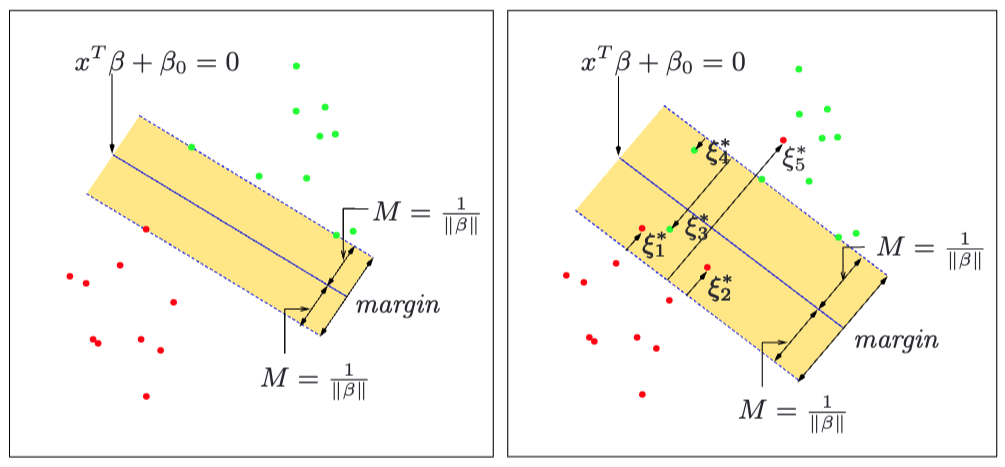
\includegraphics[width=\textwidth]{fotos/56.png}
\caption{Clasificadores de vectores de soporte. El panel izquierdo muestra el caso separable. El límite de decisión es la línea sólida, mientras que las líneas discontinuas delimitan el margen máximo sombreado de ancho $2M = 2/\|\beta\|$. El panel derecho muestra el caso no separable (superposición). Los puntos etiquetados como $\xi^*_j$ están en el lado incorrecto de su margen por una cantidad $\xi^*_j = M \xi_j$; los puntos en el lado correcto tienen $\xi^*_j = 0$, las observaciones que están en el lado incorrecto del margen tienen $\xi_j^* > 0$ y si $\xi_j^* > 1$, la observación están mal clasificada (en el lado incorrecto del hiperplano). El margen se maximiza sujeto a un presupuesto total $\sum \xi_i \leq \text{constante}$. Por lo tanto, $\sum \xi^*_j$ es la distancia total de los puntos en el lado incorrecto de su margen.}
\label{fig:12.1}
\end{figure}

Como las clases son separables, se puede encontrar una función $f(x) = x^T\beta + \beta_0$ con $y_i f(x_i) > 0 \; \forall i$. Por lo tanto, se puede encontrar el hiperplano que crea el mayor margen entre los puntos de entrenamiento para la clase 1 y -1 (ver figura \ref{fig:12.1}). El problema de optimización 
\begin{align}
\max_{\beta, \beta_0, \|\beta\|=1} & M \\
\text{sujeto a} \quad & y_i (x_i^T \beta + \beta_0) \geq M, \quad i = 1, \ldots, N
\end{align}
captura este concepto. La banda en la figura está a $M$ unidades de distancia del hiperplano en ambos lados, y por lo tanto tiene un ancho de $2M$ unidades. Se llama el margen. El conjunto de condiciones asegura que todos los puntos estén al menos a una distancia firmada $M$ del límite de decisión definido por $\beta$ y $\beta_0$, y buscamos el mayor $M$ y los parámetros asociados. Podemos deshacernos de la restricción $\|\beta\| = 1$ reemplazando las condiciones con
\begin{equation}
\frac{1}{\|\beta\|} y_i (x_i^T \beta + \beta_0) \geq M,
\end{equation}

\noindent lo que redefine $\beta_0$ o, de forma equivalente,
\begin{equation}
y_i (x_i^T \beta + \beta_0) \geq M \|\beta\|.
\end{equation}

Dado que para cualquier $\beta$ y $\beta_0$ que satisfagan estas desigualdades, cualquier múltiplo escalado positivamente también las satisface, podemos establecer arbitrariamente $\|\beta\| = \frac{1}{M}$. Así, el problema de optimización puede reformularse de manera más conveniente como
\begin{align}
\min_{\beta, \beta_0} & \frac{1}{2} \|\beta\|^2 \\
\text{sujeto a} \quad & y_i (x_i^T \beta + \beta_0) \geq 1, \quad i = 1, \ldots, N
\end{align}
\begin{align}
\min_{\beta, \beta_0} & \|\beta\| \\
\text{sujeto a} \quad & y_i (x_i^T \beta + \beta_0) \geq 1, \quad i = 1, \ldots, N
\end{align}

donde hemos eliminado la restricción de la norma en $\beta$. Nótese que $M = 1/\|\beta\|$. La expresión anterior es la forma usual de escribir el criterio de vectores de soporte para datos separados. Este es un problema de optimización convexa (criterio cuadrático, restricciones de desigualdad lineales) del cual conocemos la solución. \\

\noindent La función lagrangiana (primal), que se debe minimizar con respecto a $\beta$ y $\beta_0$, es
\begin{equation}
L_P = \frac{1}{2} \|\beta\|^2 - \sum_{i=1}^N \alpha_i [y_i (x_i^T \beta + \beta_0) - 1].
\end{equation}

\noindent Al establecer las derivadas a cero, obtenemos:
\begin{align}
\beta &= \sum_{i=1}^N \alpha_i y_i x_i \label{eq:4.50}\\
0 &= \sum_{i=1}^N \alpha_i y_i, \label{eq:4.51}
\end{align}

\noindent y sustituyendo estos en $L_P$ obtenemos el dual de Wolfe
\begin{align}
L_D =& \sum_{i=1}^N \alpha_i - \frac{1}{2} \sum_{i=1}^N \sum_{k=1}^N \alpha_i \alpha_k y_i y_k x_i^T x_k \\
& \text{sujeto a} \quad \alpha_i \geq 0 \; \text{ y } \; \sum_{i=1}^N \alpha_i y_i = 0 \label{eq:4.52}
\end{align}

Recordemos que, al ser nuestra función convexa, existe una equivalencia entre el valor óptimo del primal y del dual. La solución se obtiene maximizando $L_D$ en el ortante positivo, un problema de optimización convexa más simple, para el cual se puede usar \textit{software} estándar. Además, la solución debe satisfacer las condiciones de Karush-Kuhn-Tucker, que incluyen (\ref{eq:4.50}), (\ref{eq:4.51}), (\ref{eq:4.52}) y
\begin{equation}
\alpha_i [y_i (x_i^T \beta + \beta_0) - 1] = 0 \quad \forall i \label{eq:4.53}
\end{equation}

\noindent De estas podemos ver que
\begin{itemize}
    \item si $\alpha_i > 0$, entonces $y_i (x_i^T \beta + \beta_0) = 1$, o en otras palabras, $x_i$ está en el límite de la franja (es un vector de soporte).
    \item si $y_i (x_i^T \beta + \beta_0) > 1$, $x_i$ no está en el límite de la franja, y $\alpha_i = 0$.
\end{itemize}

De (\ref{eq:4.50}) vemos que el vector solución $\beta$ se define en términos de una combinación lineal de los puntos de soporte $x_i$, aquellos puntos definidos para estar en el límite de la franja mediante $\alpha_i > 0$. Resolviendo \ref{eq:4.53} (para cualquier vector de suporte) se obtiene $\beta_0$. Para mantener cierta estabilidad numérica, se puede promediar sobre todas las soluciones. Debemos saber calcular esto ! En general, el clasificador de máximo margen está siempre sobreaprendido. \\

Supongamos ahora que las clases se superponen en el espacio de características. Una forma de lidiar con la superposición es seguir maximizando $M$, pero permitir que algunos puntos estén en el lado incorrecto del margen. Definimos las variables de holgura $\xi = (\xi_1, \xi_2, \ldots, \xi_N)$; según su valor, podremos saber si las observaciones están en el lado correcto o incorrecto del plano (figura \ref{fig:12.1}). Hay dos formas naturales de modificar la restricció ndel problema de optimización:
\begin{equation}
y_i (x_i^T \beta + \beta_0) \geq M - \xi_i,
\end{equation}

\noindent o
\begin{equation}
y_i (x_i^T \beta + \beta_0) \geq M (1 - \xi_i),
\end{equation}

$\forall i, \xi_i \geq 0, \sum_{i=1}^N \xi_i \leq \text{constante}$. Las dos opciones conducen a soluciones diferentes. La primera opción parece más natural, ya que mide la superposición en la distancia real desde el margen; la segunda opción mide la superposición en la distancia relativa, que cambia con el ancho del margen $M$. Sin embargo, la primera opción resulta en un problema de optimización no convexa, mientras que la segunda es convexa; por lo tanto, la segunda opción conduce al ``clasificador de vectores de soporte'' estándar, que usaremos de aquí en adelante. \\

Aquí está la idea de la formulación. El valor $\xi_i$ en la restricción $y_i (x_i^T \beta + \beta_0) \geq M (1 - \xi_i)$ es la cantidad proporcional por la cual la predicción $f(x_i) = x_i^T \beta + \beta_0$ está en el lado incorrecto de su margen. Por lo tanto, al limitar la suma $\sum \xi_i$, limitamos la cantidad proporcional total por la cual las predicciones caen en el lado incorrecto de su margen. Las clasificaciones erróneas ocurren cuando $\xi_i > 1$, por lo que al limitar $\sum \xi_i$ a un valor $K$, limitamos el número total de clasificaciones erróneas de entrenamiento a $K$.
Si eliminamos la restricción de la norma en $\beta$, definir $M = 1/\|\beta\|$, podemos reescribir de nuevo el problema de optimización como 
\begin{equation}
\min \|\beta\| \quad \text{sujeto a}
\begin{cases}
y_i (x_i^T \beta + \beta_0) \geq 1 - \xi_i \quad \forall i, \\
\xi_i \geq 0, \sum \xi_i \leq \text{constante}.
\end{cases}
\label{eq:12.7}
\end{equation}

Si la constante es 0 tenemos sobreaprendizaje, mientras que si es muy grande, estamos subaprendidos. Esta es la forma usual en que se define el clasificador de vectores de soporte para el caso no separable. El panel derecho de la figura \ref{fig:12.1} ilustra este caso de superposición. \\

Por la naturaleza del criterio (\ref{eq:12.7}), vemos que los puntos bien dentro de su límite de clase no juegan un papel importante en la formación del límite. Esto parece una propiedad atractiva, y una que lo diferencia del análisis discriminante lineal. En LDA, el límite de decisión está determinado por la covarianza de las distribuciones de clase y las posiciones de los centroides de clase. La regresión logística resulta más similar al clasificador de vectores de soporte en este aspecto.

\subsection{El caso no separable}

El clasificador de máximo margen es una forma muy natural de realizar la clasificación si existe un hiperplano separador. Sin embargo, en muchos casos este hiperplano no existe, y por lo tanto no hay un clasificador de máximo margen. En este caso, el problema de optimización anterior no tiene solución con $M > 0$. Un ejemplo se muestra en la figura \ref{fig:9.4}. En este caso, no podemos separar exactamente las dos clases. Sin embargo, podemos extender el concepto de un hiperplano separador para desarrollar un hiperplano que casi separa las clases, utilizando un llamado margen suave. La generalización del clasificador de margen máximo al caso no separable se conoce como el clasificador de vectores de soporte.

\begin{figure}[h]
\centering
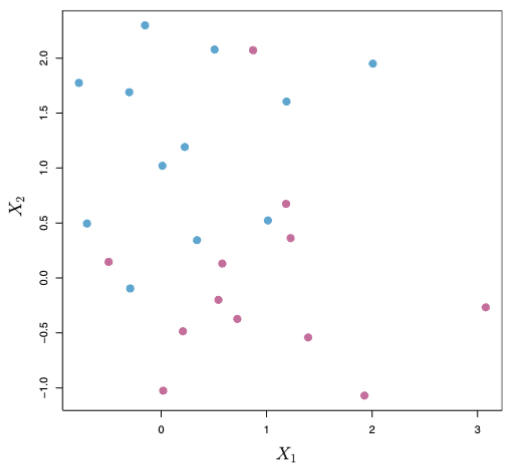
\includegraphics[width=0.5\textwidth]{fotos/55.png}
\caption{Un conjunto de datos en el que no existe un hiperplano separador.}
\label{fig:9.4}
\end{figure}








\section{Nuevo}


En ridge, con lambda 0 teniamos un metodo sobreaprendido, y en el caso de la constante muy grande era subaprendido. Para las de vectores de soporte, un C muy grande es sobreaprendido (compensa los xi yendo a 0), y un C muy pequeño es subaprendido. El papel de C es del inverso de una constante de regularización. \\


A partir de los valores de los vectores epsilon, alpha y las ec 12.10-12.16 se puede reoslver el problema que sea con los vectores de soporte. Para un vectpr sobre el margen conocemos el valor de epsilon (0). Con los vectores de soporte calculamos beta, luego para clacular beta0 tenemos algunos epsilon desconocidos (vec soporte que no estan en el margen) en este caso calculamos los beta 0 solo para los vectores que estan sobre el margen (los unicos que tenemos e un calsificador de maiximo margen) u luego hacemos la media (como antes basicamente.)

Sobre el margen: alpha mayor que 0 y menor que C, epsilon 0 y mu es mayor que 0, por lo que alpha estara entre 0 y C. Los que no estan en el margen tienen alpha igual a C porque como epsilon es distinto de 0 mu tiene que ser 0. Dentro del margen es alpha igual a C, es . El margen es la inversa del modulo de beta (no considera a beta0). SIEMPRE NOS DA LOS ALPHA Y LA C.

Para calcular las epislon de los vectores de soporte (clasificadores) hay que hacerlo conociendo beta 0 y beta. Esto da la distancia en unidades del margen 


El signo dice la clase (+ a +1 y - a -1) y la magnitud la distancia al hiperplano



C COMO PARAMETRO
C muy pequeño, permitimos mucho epsilon alto y por tant oestamos en subaprendizaje y habra muchos vectores de soporte. Si C es muy grande, estamos en sobreaprendizaje y habra muy pocos vectores de soporte. Similar a KNN. \\



hasta ahora al hablar de vectores de soporte hablamos de CALSIFICADORES, NO MAQUINA